% -------请使用xelatex编译------- %
\documentclass{sysu_report}
\title{中山大学实验报告模板——使用教程}
\def\school{XXXXXX} % 院系
\def\major{XXXXXX}  % 专业
\author{XXXXXX}                   % 姓名
\def\id{20260000000}            % 学号
\def\location{XXXXXX}    % 实验地点
\def\instructor{XXXXXX}           % 指导教师
\date{\today}
\begin{document}
\maketitle
{
\hypersetup{linkcolor=black}
\setlength{\parskip}{0pt}
\tableofcontents
}
\clearpage
\setcounter{page}{1}
\renewcommand{\thepage}{\arabic{page}}
\maintext%
% -------以下为正文------- %
\section{封面与基本信息}
本模板基于 \texttt{ctexart} 文档类，使用 XeLaTeX 编译，已默认配置好中英文字体、页边距、行距、页眉页脚等排版细节。配置文件为 \texttt{sysu\_report.cls}。
下面从封面设置开始，逐步介绍模板的各项功能。\par
\subsection{封面信息填写}
封面由 \verb|\maketitle| 自动生成，你需要填写以下信息：\par
\begin{itemize}
    \item \verb|\title{标题}| —— 实验报告标题
    \item \verb|\def\school{院系}| —— 所在院系名称
    \item \verb|\def\major{专业}| —— 专业名称
    \item \verb|\author{姓名}| —— 你的姓名
    \item \verb|\def\id{学号}| —— 学号
    \item \verb|\def\location{地点}| —— 实验地点
    \item \verb|\def\instructor{教师}| —— 指导教师姓名
\end{itemize}\par
封面自动包含中山先生提笔的中山大学校名（\texttt{fig/SYSU\_logo.pdf}），请确保该文件存在。
封面排版风格为仿宋加粗标题与楷体个人信息，符合习惯样式。\par
\subsection{目录生成}
使用 \verb|\tableofcontents| 即可自动生成目录。
模板已设置目录显示深度为 4 级，对应 \verb|\section|、\verb|\subsection|、\verb|\subsubsection| 和 \verb|\paragraph|。
目录中的引导线为点线，页码自动对齐。\par
模板默认给目录中的链接颜色单独设置为黑色（\verb|linkcolor=black|），以避免目录页出现大片彩色链接。
正文中的交叉引用则为道奇蓝色（Dodger Blue）。
\section{正文排版——标题层级与字体}
\subsection{标题层级}
模板提供了四级标题，均使用黑体加粗（\verb|\hei\bfseries|），由 \texttt{titlesec} 宏包控制格式：
\begin{itemize}
    \item \verb|\section{一级标题}| —— 居中、小二号字，每个 section 自动另起一页
    \item \verb|\subsection{二级标题}| —— 左对齐、四号字
    \item \verb|\subsubsection{三级标题}| —— 左对齐、小四号字
    \item \verb|\paragraph{段落标题}| —— 左对齐、小四号字
\end{itemize}
\subsubsection{小标题示例}
这是一个三级标题示例，使用 \verb|\subsubsection| 定义。你可以在正文中任意位置使用这些标题命令，模板会自动处理编号和格式并纳入目录。
\paragraph{段落标题示例}
这是一个段落示例，使用 \verb|\paragraph| 定义，该级标题也会出现在目录中。
模板通过 \verb|\setcounter{secnumdepth}{4}| 和 \verb|\setcounter{tocdepth}{4}| 确保所有四级标题均编号并纳入目录。
\subsection{正文字体与样式}
模板正文默认使用宋体（FandolSong）、小四号字、首行缩进两字符、段间距为零。
这些设置在 \verb|\maintext| 命令中完成，该命令应在正文开始处调用一次。否则样式将变为 \verb|ctexart| 默认样式，那将十分不好看。:(\par
正文默认行距设置为 1.625 倍（对应 Word 中的 1.5 倍行距），页边距为上下 2.5cm、左右 3cm。\par
在\LaTeX{}中，如果你想让文字分段，直接在文本中用两次回车让段落间空一行或直接使用 \verb|\par| 命令即可。如果你发现你的正文某段突然没有了缩进，
通常是因为你在其上段使用了类似于 \verb|\begin{itemize}| 的环境，而没有在其环境的结束 \verb|\end{itemize}| 后面空一行或使用 \verb|\par| 命令。
顺带一提，代码中常见的 \verb|\\| 也是换行的一种，但其为强制换行，不会重制环境，请尽量只在表格中使用它。

另外，模板提供了四种中文字体的切换命令方便使用：
\begin{itemize}
    \item \verb|\song| —— {\song{}宋体（默认正文）}
    \item \verb|\kai|  —— {\kai{}楷体}
    \item \verb|\hei|  —— {\hei{}黑体（标题字体）}
    \item \verb|\fang| —— {\fang{}仿宋（页眉字体）}
\end{itemize}\par
英文字体方面，衬线体使用 Times New Roman，无衬线体为 Arial，等宽字体为 Courier New。\par
\subsection{自定义颜色}
模板引入了 \texttt{xcolor} 宏包并预定义了几个实用颜色，你也可以自行定义新颜色：
\begin{lstlisting}[language=TeX]
% 使用\definecolor{名称}{模型}{色值}自定义颜色
\definecolor{MSBlue}{RGB}{52, 90, 138}  % RGB 模型
\definecolor{myblue}{HTML}{1E90FF}      % HTML 十六进制模型
\end{lstlisting}
预定义的 \texttt{myblue}（道奇蓝）用于超链接颜色，\texttt{codeBg}（浅灰 \#F2F2F2）用于代码块背景。
你可以在正文中直接使用 \verb|\textcolor{myblue}{文字}| 得到 {\color{myblue} 蓝色文字}，
以及用 \verb|\colorbox{codeBg}{背景}| 得到 \colorbox{codeBg}{灰色背景}。
\section{数学公式与定理环境}
模板基于 \texttt{amsmath}、\texttt{amssymb}、\texttt{mathrsfs}、\texttt{amsthm} 等宏包提供了完整的数学排版支持。
\subsection{常用公式环境}
行内公式使用 \verb|$...$|，如 $E = mc^2$。行间公式推荐使用 \verb|equation| 环境，编号格式为``章-序号''，每节重新计数：
\begin{equation}
    \mathcal{F}(\omega) = \int_{-\infty}^{+\infty} f(t) e^{-j\omega t} \, dt
    \label{eq:fourier}
\end{equation}\par
公式 \eqref{eq:fourier} 是连续傅里叶变换的定义式。多行对齐可使用 \texttt{align} 环境：
\begin{align}
    \frac{\partial u}{\partial t} &= \alpha \nabla^2 u \label{eq:heat1} \\
    \nabla^2 &= \frac{\partial^2}{\partial x^2} + \frac{\partial^2}{\partial y^2} + \frac{\partial^2}{\partial z^2} \label{eq:laplacian}
\end{align}\par
带括号的矩阵、分段函数等复杂结构也都完整支持：
\begin{equation}
    \mathbf{A} = \begin{pmatrix}
        a_{11} & a_{12} & \cdots & a_{1n} \\
        a_{21} & a_{22} & \cdots & a_{2n} \\
        \vdots & \vdots & \ddots & \vdots \\
        a_{m1} & a_{m2} & \cdots & a_{mn}
    \end{pmatrix}
    \label{eq:matrix}
\end{equation}
\subsection{定理类环境}
模板预定义了以下定理环境（由 \texttt{amsthm} 提供），均按章编号：
\begin{definition}[环]
    设 $R$ 是一个非空集合，在其上定义了两种二元运算``加法''和``乘法''，若满足 $(R,+)$ 是交换群、$(R,\cdot)$ 是半群、且乘法对加法满足分配律，则称 $R$ 为一个\textbf{环}。
    \label{def:ring}
\end{definition}

\begin{thm}[柯西中值定理]
    设函数 $f(x)$ 和 $g(x)$ 在闭区间 $[a,b]$ 上连续，在开区间 $(a,b)$ 内可导，且 $g'(x) \neq 0$，则存在 $\xi \in (a,b)$ 使得
    \begin{equation}
        \frac{f(b) - f(a)}{g(b) - g(a)} = \frac{f'(\xi)}{g'(\xi)}
    \end{equation}
    \label{thm:cauchy}
\end{thm}

\begin{lemma}[Gronwall 不等式]
    设 $u(t)$ 和 $\alpha(t)$ 是 $[t_0, t_1]$ 上的连续函数，$\beta(t) \geq 0$ 在 $[t_0, t_1]$ 上可积。若
    $u(t) \leq \alpha(t) + \int_{t_0}^{t} \beta(s) u(s) \, ds$，则有
    \begin{equation}
        u(t) \leq \alpha(t) + \int_{t_0}^{t} \alpha(s)\beta(s) \exp \bigl(\int_{s}^{t}\beta(r)\,dr\bigr)\,ds
    \end{equation}
    \label{lem:gronwall}
\end{lemma}

\begin{corollary}[零点存在定理]
    若连续函数 $f$ 在 $[a,b]$ 上有 $f(a)f(b) < 0$，则存在 $c \in (a,b)$ 使得 $f(c) = 0$。
    \label{cor:zero}
\end{corollary}

\begin{remark}
    推论~\ref{cor:zero}~是定理~\ref{thm:cauchy}~中取 $g(x) = x$ 的特殊情况，也是连续函数介值定理的直接结论。
\end{remark}

\begin{proof}[定理~\ref{thm:cauchy}~的证明概要]
    构造辅助函数 $h(x) = [f(b)-f(a)]g(x) - [g(b)-g(a)]f(x)$，验证 $h(a)=h(b)$，由罗尔定理即得结论。
\end{proof}

以上定理、定义、引理、推论、注和证明环境均继承了标准 \LaTeX{} 的语义化标记习惯，在撰写数学类或理论分析类实验报告时非常实用。
\section{图片与表格}
\subsection{插入图片}
使用 \verb|\includegraphics| 插入图片，配合 \texttt{figure} 浮动环境和 \verb|\caption| 生成图题。图题使用黑体小四号字，编号格式为``章-序号''。

\begin{figure}[H]
    \centering
    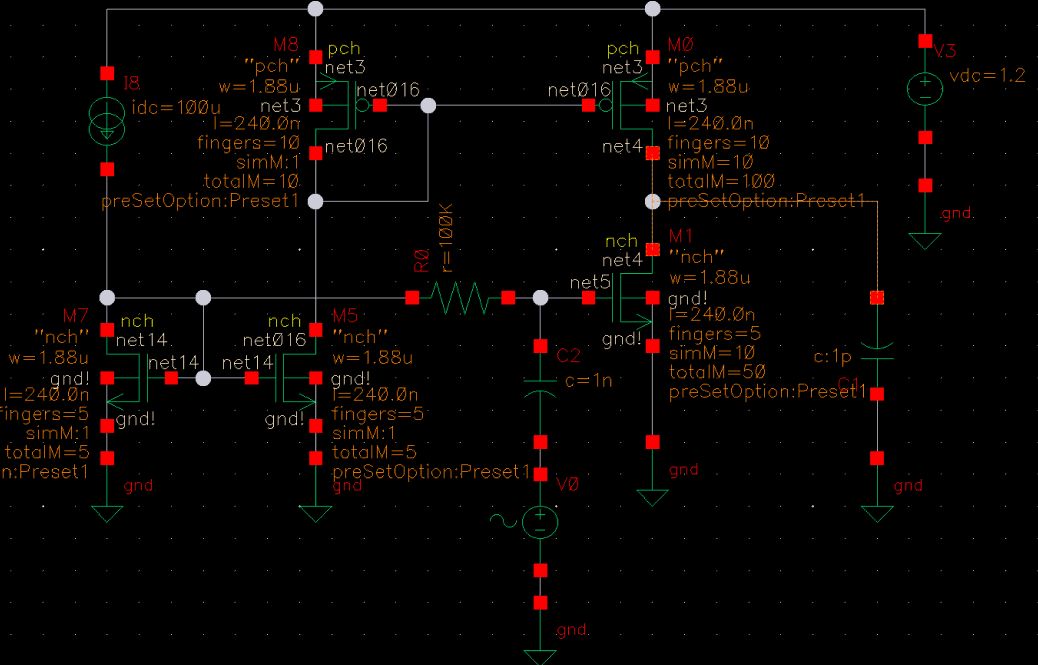
\includegraphics[width=0.65\textwidth]{fig/example_circuit.png}
    \caption{共源极放大电路原理图}
    \label{fig:circuit}
\end{figure}

图~\ref{fig:circuit}~展示了一共源极放大电路的结构，其中 \verb|[width=0.65\textwidth]| 可控制图片宽度。
在行文中如果需要引用图片，你可以使用 \verb|\label{fig:xxx}| 标记图片，再用 \verb|\ref{fig:xxx}| 引用编号。注意图题中的编号会自动加上当前 section 前缀。\par
插入多张并列图片时，有三种常用方法：
\subsubsection{方法一：直接并列}
最简单的做法是连续使用 \verb|\includegraphics|，在中间使用 \verb|\hspace| 或 \verb|\hfill| 隔开图片：

\begin{figure}[H]
    \centering
    \includegraphics[width=0.45\textwidth]{fig/example_dc.bmp}
    \hspace{0.05\textwidth}
    \includegraphics[width=0.45\textwidth]{fig/example_ro.bmp}
    \caption{直流仿真（左）与输出阻抗（右）——直接并列}
    \label{fig:side_by_side}
\end{figure}

\subsubsection{方法二：minipage 环境}
用 \texttt{minipage} 可以给每张图独立的标题或说明文字，适合子图需要分别标注的场景：

\begin{figure}[H]
    \centering
    \begin{minipage}{0.45\textwidth}
        \centering
        \includegraphics[width=\textwidth]{fig/example_dc.bmp}
        \caption{直流仿真曲线}
        \label{fig:dc}
    \end{minipage}
    \hspace{0.05\textwidth}
    \begin{minipage}{0.45\textwidth}
        \centering
        \includegraphics[width=\textwidth]{fig/example_ro.bmp}
        \caption{输出阻抗曲线}
        \label{fig:ro}
    \end{minipage}
\end{figure}

\subsubsection{方法三：subcaption 宏包}
模板已加载 \texttt{subcaption} 宏包，使用 \texttt{subfigure} 环境是推荐做法——共享主图题，
每张子图有独立子编号（(a)、(b) \ldots），交叉引用更规范：

\begin{figure}[H]
    \centering
    \begin{subfigure}{0.45\textwidth}
        \centering
        \includegraphics[width=\textwidth]{fig/example_dc.bmp}
        \caption{直流仿真}
        \label{fig:sub_dc}
    \end{subfigure}
    \hspace{0.05\textwidth}
    \begin{subfigure}{0.45\textwidth}
        \centering
        \includegraphics[width=\textwidth]{fig/example_ro.bmp}
        \caption{输出阻抗}
        \label{fig:sub_ro}
    \end{subfigure}
    \caption{直流仿真与输出阻抗对比（subcaption 方式）}
    \label{fig:subcaption_demo}
\end{figure}

三种方式各有用处：方法一最轻量；方法二适合子图需要各自独立图题时；方法三最规范，推荐在正式报告中使用，
引用子图时用 \verb|\ref{fig:sub_dc}| 即可得到类似``~\ref{fig:sub_dc}~''的编号。
\subsection{插入表格}
表格使用 \texttt{tabularx}（自适应列宽）配合 \texttt{booktabs} 三线表风格。模板定义了三种便捷列类型：\texttt{L}（左对齐）
、\texttt{C}（居中）、\texttt{R}（右对齐），比传统的 \texttt{l/c/r} 更灵活。表题同样使用黑体小四号字。

\begin{table}[H]
    \centering
    \caption{共源极放大电路——静态工作点测量数据}
    \label{tab:dc_op}
    \begin{tabularx}{0.85\textwidth}{CCCC}
        \toprule
        $V_{GS}$ (V) & $V_{DS}$ (V) & $I_D$ (mA) & $g_m$ (mS) \\
        \midrule
        1.50 & 5.12 & 2.34 & 4.68 \\
        1.80 & 4.87 & 3.01 & 5.21 \\
        2.10 & 4.55 & 3.78 & 5.89 \\
        2.40 & 4.20 & 4.62 & 6.43 \\
        \bottomrule
    \end{tabularx}
\end{table}

表~\ref{tab:dc_op}~展示了不同偏置电压下的静态工作点。接下来展示一个稍微复杂一点的表格，使用 \verb|\makecell| 实现表头换行：

\begin{table}[H]
    \centering
    \caption{放大器性能参数实测值}
    \label{tab:ac_params}
    \begin{tabularx}{0.9\textwidth}{CCCCC}
        \toprule
        \makecell[cc]{频率\\(kHz)} & \makecell[cc]{电压增益\\$A_v$ (dB)} & \makecell[cc]{输入阻抗\\$Z_{in}$ ($\Omega$)} & \makecell[cc]{输出阻抗\\$Z_{out}$ ($\Omega$)} & \makecell[cc]{带宽\\$BW$ (MHz)} \\
        \midrule
        1   & 18.4 & 10.2k & 2.15k &  --  \\
        10  & 18.1 &  9.8k & 2.18k &  --  \\
        100 & 17.3 &  9.1k & 2.22k &  --  \\
        1M  & 14.8 &  7.6k & 2.45k & 6.82 \\
        \bottomrule
    \end{tabularx}
\end{table}

\section{代码高亮}
模板使用 \texttt{listings} 宏包提供代码高亮。默认样式为灰底（\texttt{codeBg} 颜色）、左侧行号、单线边框、长行自动换行。
关键字为蓝色，注释为绿色，字符串为红色。你也可以通过参数自定义样式，如调整颜色、字体、行距等。
\subsection{通用代码（默认样式）}
对于不预设语言的通用代码，直接使用 \verb|\begin{lstlisting}| 即可，显示效果如下。
你也可以用 \verb|language| 参数指定语言（如 C、Python、Java 等，\texttt{listings} 内置支持的语言均可使用）。

\begin{lstlisting}[language=C, caption={冒泡排序 C 语言实现}]
#include <stdio.h>

void bubble_sort(int arr[], int n) {
    for (int i = 0; i < n - 1; i++) {
        for (int j = 0; j < n - 1 - i; j++) {
            if (arr[j] > arr[j + 1]) {
                int temp = arr[j];
                arr[j] = arr[j + 1];
                arr[j + 1] = temp;
            }
        }
    }
}
\end{lstlisting}

\subsection{Arduino 代码}
模板专门定义了 Arduino 语法高亮（语言名 \texttt{Arduino}），对数据类型（蓝绿色加粗）、控制流与库函数（橙色）、
常量（橙色加粗）等进行了分类着色，适合嵌入式与物联网类实验报告。

\begin{lstlisting}[language=Arduino, caption={Arduino 读取 DHT11 温湿度传感器}]
#include <DHT.h>

#define DHTPIN 2
#define DHTTYPE DHT11

DHT dht(DHTPIN, DHTTYPE);

void setup() {
    Serial.begin(9600);
    dht.begin();
}

void loop() {
    delay(2000);
    float humidity = dht.readHumidity();
    float temperature = dht.readTemperature();

    if (isnan(humidity) || isnan(temperature)) {
        Serial.println("Failed to read from DHT sensor!");
        return;
    }
    Serial.print("Humidity: ");
    Serial.print(humidity);
    Serial.print(" %\t");
    Serial.print("Temperature: ");
    Serial.print(temperature);
    Serial.println(" *C");
}
\end{lstlisting}

\subsection{MATLAB 代码}
模板同样定义了 MATLAB 增强语法高亮（语言名 \texttt{Matlabcs}），关键字为蓝色加粗、注释为绿色、字符串为紫色，
并额外加入了 \texttt{parfor}、\texttt{table}、\texttt{readtable} 等常用高级函数的关键字。

\begin{lstlisting}[language=Matlabcs, caption={MATLAB 信号频谱分析示例}]
% 生成含噪声的正弦信号并绘制频谱
fs = 1000;            % 采样频率 (Hz)
t = 0:1/fs:1-1/fs;   % 时间向量
f0 = 50;              % 信号频率 (Hz)
x = sin(2*pi*f0*t) + 0.5*randn(size(t)); % 含噪信号

N = length(x);
X = fft(x);
f = (0:N-1)*(fs/N);   % 频率轴
magnitude = abs(X)/N; % 幅度谱

plot(f(1:N/2), magnitude(1:N/2));
xlabel('Frequency (Hz)');
ylabel('Magnitude');
title('Single-Sided Amplitude Spectrum');
grid on;
\end{lstlisting}

\section{列表与脚注}
\subsection{列表环境}
模板通过 \texttt{enumitem} 宏包压缩了列表环境的行间距，使得 \texttt{itemize}和\\
 \texttt{enumerate} 的排版更加紧凑。\par
无序列表示例如下：

\begin{itemize}
    \item 实验前需预习相关内容，明确实验目的与步骤
    \item 实验过程中记录原始数据，不得事后补填
    \item 实验报告需独立完成，严禁抄袭
\end{itemize}

有序列表的用法与标准 \LaTeX{} 一致：

\begin{enumerate}
    \item 搭建共源极放大电路，检查偏置电压是否正常
    \item 输入 1kHz 正弦波，用示波器观察输出波形
    \item 改变输入信号幅度，记录输出波形变化
    \item 测量中频电压增益，计算 -3dB 带宽
\end{enumerate}

嵌套列表同样支持，且行间距保持紧凑：

\begin{enumerate}
    \item 仪器连接
    \begin{enumerate}
        \item 信号发生器接放大器输入端
        \item 示波器通道 1 接输入端，通道 2 接输出端
        \item 直流电源接放大器供电端
    \end{enumerate}
    \item 数据采集
    \begin{itemize}
        \item 记录不同频率下的输入输出电压幅值
        \item 注意输出波形不能出现明显失真
        \item 每组数据至少重复测量三次
    \end{itemize}
\end{enumerate}

\subsection{脚注}
脚注按页编号\footnote{这是第一页的脚注，用于补充说明正文中的细节。}，使用 \verb|\footnote{文字}| 即可\footnote{每页的脚注独立编号。}。
模板的脚注计数器绑定到页码，每页重新从 1 开始。

\section{附录与参考文献}
\subsection{附录}
模板使用 \texttt{appendix} 宏包，通过 \verb|\begin{appendices}| 进入附录模式。附录中的章节自动以字母编号（附录 A、附录 B……），
且图表公式的编号也会相应切换。\par
附录也和正文一样支持标题层级、数学公式、图表等内容，适合放置实验原始数据记录表、仿真代码等补充材料。
\subsection{参考文献}
模板使用 \texttt{natbib} 宏包管理参考文献（\texttt{numbers} 模式），参考文献条目存放在 \texttt{cite.bib} 文件中。
自定义了上标引用，引用命令包括：

\begin{itemize}
    \item \verb|\cite{key}| —— 带括号引用，如 \cite{razavi2005design}
    \item \verb|\citenum{key}| —— 纯数字引用，如 \citenum{sze2021physics}
    \item \verb|\citet{key}| —— 文本内引用，如 \citet{2003A}
    \item \verb|\upcite{key}| —— 纯括号上标引用，如 \upcite{华明清20070}
    \item \verb|\upcitenum{key}| —— 纯数字上标引用，如 \upcitenum{razavi2005design}
    \item \verb|\upcitet{key}| —— 文本内引用，如 \upcitet{2003A}
\end{itemize}\par

参考文献列表标题使用黑体二号居中，条目间行距已压缩（\verb|\bibsep=0pt|）。
在正文末尾使用 \verb|\bibliographystyle{unsrtnat}| 选择引文格式，再用\\ \verb|\bibliography{cite}| 载入 bib 文件即可自动生成参考文献列表。\par
至此，本教程已覆盖模板的全部核心功能，包括封面设置、标题层级、字体切换、数理公式与定理环境、图表插入、代码高亮
（通用、Arduino、MATLAB）、列表脚注、附录以及参考文献引用。更多 \LaTeX{} 进阶用法，请自行学习。
% --------------参考文献-------------- %
\bibliographystyle{unsrtnat}
\bibliography{cite}
% --------------附录-------------- %
\begin{appendices}
\section{实验原始数据记录表}
以下为实验过程中记录的原始数据（部分摘录），供参考核对。

\begin{table}[H]
    \centering
    \caption{原始数据记录（摘录）}
    \begin{tabularx}{0.9\textwidth}{CCCC}
        \toprule
        频率 (Hz) & $V_{in}$ (mV) & $V_{out}$ (V) & 增益 $A_v$ \\
        \midrule
        100  & 50 & 0.43 & 8.6  \\
        500  & 50 & 0.45 & 9.0  \\
        1k   & 50 & 0.46 & 9.2  \\
        10k  & 50 & 0.44 & 8.8  \\
        \bottomrule
    \end{tabularx}
\end{table}

\subsection{附录标题示例}
这是一个附录中的标题示例，使用 \verb|\subsection| 定义。附录中的标题层级与正文完全一致，且会自动纳入目录。
\subsubsection{附录小标题示例}
这是一个附录中的小标题示例，使用 \verb|\subsubsection| 定义。附录中的标题层级与正文完全一致，且会自动纳入目录。
\paragraph{附录段落示例}
这是一个附录中的段落示例，使用 \verb|\paragraph| 定义。附录中的标题层级与正文完全一致，且会自动纳入目录。
\section{MATLAB 仿真代码}

\begin{lstlisting}[language=Matlabcs]
% 绘制放大器频率响应曲线
f = logspace(1, 6, 1000);  % 1Hz ~ 1MHz
Av = 20 * log10(10 ./ sqrt(1 + (f/1e5).^2));
semilogx(f, Av, 'LineWidth', 1.5);
xlabel('Frequency (Hz)');
ylabel('Gain (dB)');
grid on;
\end{lstlisting}

\end{appendices}

\end{document}